%\bibliography{/home/jorgsk/phdproject/bibtex/jorgsk}
Transcription is the synthesis of a complementary RNA molecule from a DNA
template. The macromolecule that performs transcription is the DNA-dependent
RNA polymerase (RNAP). See Figure \ref{fig:transcription_elongation} for an
overview of transcription elongation by RNA polymerase.

\begin{figure}[htb]
    \begin{center}
        \includegraphics[scale=0.6]{illustrations/sysbio/1_normal_transcription.pdf}
    \end{center}
    \caption{Transcription elongation by RNA polymerase. The nascent RNA
    transcript grows at the 3\protect\ppp end where NTP binds and is
    incorporated into the RNA nucleotide chain. NTP binds in a complementary
    fashion to bases on the single stranded template DNA which are exposed due
    to the $\sim$ 14/15 bp DNA transcription bubble.}
    \label{fig:transcription_elongation}
\end{figure}

In bacteria, RNAP consists of the subunits $\beta$, $\beta^{\prime}$, $\omega$,
and two $\alpha$ subunits and has a molecular mass of around 400 kDa. The
structure and function of bacterial RNAPs are conserved in comparison with
archaea and eukaryotes \cite{borukhov_rna_2008}, showing that the fundamental
mechanism of RNA synthesis is the same for all cell types.

Here, we will review the role of RNAP in initiation, elongation, and
termination of transcription in bacteria. Special care will be given to the
topic of abortive transcription initiation and how RNAP moves along DNA during
transcription.

\subsubsection{Promoter localization}
Before RNAP can start transcription of a gene it must localize a transcription
start site (TSS). These sites are advertised by promoters, stretches of DNA
which are typically located from around -60 to +20 basepairs relative to the
TSS \cite{ross_third_1993,hsu_promoter_2002}. RNAP cannot bind strongly to
promoters directly, but must first associate with a regulatory protein called
sigma ($\sigma$) factor; the $\sigma$ factor in turn only binds strongly to
promoters when in complex with RNAP \cite{paget_<sup>70</sup>_2003}, making
the RNAP-$\sigma$ complex essential for transcription initiation. In
\textit{E.\ coli} there are seven types of $\sigma$ factors, where each
$\sigma$ factor regulates the binding of RNAP to promoters associated with a
particular gene family \cite{osterberg_regulation_2011}. For example,
$\sigma^{70}$ recognizes promoters for housekeeping genes, while $\sigma^{32}$
recognizes promoters for genes that are activated in conditions of heat shock.
Most promoters are of the $\sigma^{70}$ type (meaning that $\sigma^{70}$ binds
to them), and we will here focus on this type of promoter. The most prominent
$\sigma$-binding elements in $\sigma^{70}$ promoters are the -35 and -10
hexamer (six-nucleotide) motifs, with the consensus sequences TTGACA (-35) and
TATAAT (-10) \cite{ross_analysis_2009}. The major determinant for how strongly
$\sigma^{70}$ binds to a promoter is how much the -35 and -10 motifs vary from
the consensus, as well as the distance in nucleotides between these elements.
A third sequence that can affect promoter-RNAP-$\sigma^{70}$ binding is an AT
rich element upstream -35 called, simply, the upstream element
\cite{ross_third_1993, haugen_fine_2008} (see Figure \ref{fig:promoter}). In
general, the stronger $\sigma^{70}$ binds to a promoter the higher the
transcription initiation rate will be, which again may lead to higher
expression of the downstream gene.  However, we will shortly see that the
initial transcribed sequence, defined as the region from +1 to +20 realtive to
the TSS (Figure \ref{fig:promoter}), may also influence the expression from a
promoter.

\begin{figure}[htb]
	\begin{center}
		\includegraphics[scale=0.5]{illustrations/promoter_its.pdf}
	\end{center}
	\caption{RNAP and sigma bound to promoter elements. Positions along the DNA
	template are indicated relative to the transcription start site.}
	\label{fig:promoter}
\end{figure}

\subsubsection{Transcription initiation}
% nucleotide = base-sugar-phosphate (1 or 3)
% nucleoside = base-sugar
% BUT! this confusing terminology exists: ``nucleotide with 3 phosphates'' =
% nucleoside triphosphate.
Once the RNAP-$\sigma$ complex has bound to a promoter, transcription
initiation may commence. First, $\sigma$ mediates the opening of the double
stranded DNA from -11 to +2 \cite{borukhov_rna_2008}. The unwound DNA helix is
referred to as the DNA bubble, or the transcription bubble. Within the DNA
bubble, bases on the template DNA strand are exposed and ready to base pair
with incoming NTP. After having opened the DNA bubble, RNAP is positioned so that the
nucleotide at the TSS is at RNAP's active site (the active site is the part of
RNAP where RNA synthesis occurs). When transcription begins, the two first
nucleotides bind in the active site and a phosphodiester bond is formed between
them \cite{mcclure_steady_1978}. This constitutes the first dinucleotide of
the nascent RNA. In order to incorporate the third nucleotide, RNAP must first
move its active site relative to downstream DNA to make room for the incoming
NTP. However, RNAP is bound to the promoter, making it immobile. It can
therefore not translocate downstream as it would during transcription
elongation. Instead, translocation during initiation results in RNAP pulling
DNA into itself in a process that has been labeled ``scrunching''
\cite{kapanidis_initial_2006, revyakin_abortive_2006}.  By pulling in
downstream DNA, RNAP's active site translocates relative to template DNA,
making the active site available for incoming NTP, even though RNAP is still
bound to the upstream promoter sequence. A consequence of scrunching is that
the DNA bubble increases in size with 1bp for each scrunching step, since one
basepair of DNA is opened downstream without the complementary closing of an
upstream basepair as for transcription elongation. The increasingly large DNA
bubble that results from scrunching has been suggested to play a role for both
promoter escape and abortive RNA release \cite{hsu_promoter_2002,
kapanidis_initial_2006}.

Transcription initiation proceeds in a cycle of scrunching, NTP binding, and
phosphodiester bond formation. With each step, the DNA bubble grows with one
basepair and the nascent RNA grows with one nucleotide. When the nascent RNA
reaches a length of around 10-12 nt, promoter escape may occur if $\sigma$
dissociates from the promoter \cite{hsu_promoter_2002} (see
Figure \ref{fig:simple_escape}).

\begin{figure}[htb]
	\begin{center}
		\includegraphics[scale=0.5]{illustrations/sysbio/7_transcription_initiation.pdf}
	\end{center}
	\caption{Promoter escape involves scrunching of DNA.}
	\label{fig:simple_escape}
\end{figure}

\subsubsection{Abortive initiation}
Promoter escape is, however, only one outcome of a transcription initiation
attempt. Another outcome is that the initiation attempt fails, which means that
the nascent RNA is released prematurely before promoter escape can occur
\cite{early_cycling_paper_1982}. The
starting point of a failed initiation attempt is a reversal of the
translocation-scrunching reaction, a step which is referred to as backtracking
\cite{hsu_initial_2006}. When backtracking occurs, the ``unschrunching`` of
DNA forces the 3\ppp end of the nascent RNA into the entry channel for NTP,
leading to a shortened RNA-DNA hybrid \cite{hsu_initial_2006}. Eventually the
nascent RNA is released from this complex, possibly because the shortened
RNA-DNA hybrid is unstable. RNA release is assumed to be accompanied by a
release of the rest of the scrunched DNA from RNAP, since it is known that
after an abortive RNA release RNAP can fall back to the open complex
formation, where it may restart transcription initiation \textit{de novo}
\cite{hsu_promoter_2002} (see Figure \ref{fig:abortive_backtrack}).

\begin{figure}[htb]
	\begin{center}
		\includegraphics[scale=0.5]{illustrations/sysbio/8_transcription_initiation_backtracking.pdf}
	\end{center}
	\caption{Abortive initiation caused by a backtracking-``unscrunching''
	reaction.}
	\label{fig:abortive_backtrack}
\end{figure}

The term for unscrunching and RNA release during transcription initiation is
abortive initiation. A related term is abortive cycling, which refers to
repeated initiation attempts that end with abortive RNA release (see Figure
\ref{fig:abortive_cycling}). The aborted RNA fragments are generally no longer
than 15 nucleotides, but lengths up to 20 have been observed
\cite{chander_alternate_2007}. In \textit{in vitro} experiments abortive
initiation is the rule rather than the exception for many promoters
\cite{hsu_promoter_2002}. Some promoters have a calculated \textit{in vitro}
ratio of aborted to successful transcription initiation attempts of over 300
\cite{hsu_initial_2006}. This indicates that RNAP may on average spend
considerable time in abortive cycling before achieving promoter escape.

\begin{figure}[htb]
	\begin{center}
		\includegraphics[scale=0.4]{illustrations/sysbio/9_abortive_cycling.pdf}
	\end{center}
	\caption{Repeated abortive RNA release and \textit{de novo} transcription
	initiation is called abortive cycling.}
	\label{fig:abortive_cycling}
\end{figure}

\subsubsection{Experimental detection of abortive initiation}
To quantify abortive initiation, one must obtain a measure of the molar
abundance of each abortive RNA while ensuring that abortive RNAs of a given
length are quantified separately from any possible cleavage product of the same
length (since a backtracked RNA can be cleaved at the RNAP active site before
abortive release occurs). A method that fulfills these two requirements is
radioactive labeling using nucleotide $\gamma$-phosphates
\cite{hsu_monitoring_2009}. Each abortive RNA will only contain one
$\gamma$-phosphate, namely the one at the 5\ppp end. All other
$\gamma$-phosphates are cleaved off during transcription and released in
pyrophosphate (PPi). By separating abortive RNAs in terms of their length on a
single-nucleotide resolution gel, one can then use a phosphoimager to quantify
the amount of each abortive product \cite{hsu_monitoring_2009}. By this method,
one can infer at which nucleotide positions abortive initiation occurs and to
what extent \cite{hsu_<i>vitro</i>_2003}. Although cleaved RNA is contained in
the gel, the lack of a radioactive phosphate means it will not affect the
quantification of abortive RNAs.

\subsubsection{Calculation of abortive probability}
The quantification of abortive RNAs of different lengths permits the
calculation of abortive probability (AP) at each template position, as
described by Hsu \cite{Lilian_AP_note_95}. Briefly, the probability to abort a
transcript of length $i$ is given as 
\begin{equation*}
    \frac{R_i}{P_i},
\end{equation*}
where $R_i$ is the number of abortive RNAs of length $i$ and $P_i$ is the
number of polymerases that transcribe to reach an RNA of length $i$. This can
be written as
\begin{equation*}
    \frac{R_i}{P_i} = \frac{r_iR}{p_iP}.
\end{equation*}
Here, $r_i$ is the fraction of RNAs of length $i$ in terms of total RNA ($R$),
and $p_i$ is the fraction of RNAPs transcribing an RNA of length $i$ in terms
of total RNAPs ($P$). We assume that each observed aborted RNA corresponds to
one transcribing RNAP, so that $R = P$. Therefore, we find the abortive
probability as 
\begin{equation*}
    AP_i = \frac{r_i}{p_i}.
\end{equation*}

The fraction of abortive RNAs of each length is found directly from the
phosphoimaging quantification. The fraction of RNAP obtaining an RNA of length
$i$ is found iteratively in the following way: 100\% of RNAPs obtain an RNA of
length 2; if for example 40\% of all abortive RNA is of length 2, then we know
that 60\% of RNAPs obtain an RNA of length 3; then, if for example 15\% of all
abortive RNA is of length 3, then we know that 45\% of RNAPs obtain an RNA of
length 4; and so on.

\subsubsection{Promoter escape and the initial transcribed sequence}
An early discovery by Kammerer et al.\ \cite{kammerer_functional_1986} was that
the promoter sequence downstream +1 can have a strong effect on promoter
strength.  Kammerer et al.\ found this effect by comparing the promoter
strength of the N25 phage promoter with a variant of N25 constructed by changing C
for A, T for G and vice versa for N25's +1 to +20 sequence. This variant was
called N25/anti, and has later been referred to as N25$_{\text{anti}}$
\cite{hsu_<i>vitro</i>_2003}. Later, it was found that the cause for the difference
in promoter strength was due to a large increase in both the amount and length
of abortive transcripts produced from N25/anti compared to N25
\cite{hsu_<i>escherichia_1995, hsu_<i>vitro</i>_2003}. To comprehensively map
the effect of the +1 to +20 sequence on promoter escape, Hsu et al.\
\cite{hsu_initial_2006} investigated \textit{in vitro} the abortive properties
of a library of 43 promoter variants which had randomized +1 to +20 initial
transcribed sequences (ITSs). They showed that sequence variation in the ITS
could result in a 20-fold difference in promoter escape efficiencies. In the
study by Hsu et al.\, promoter escape efficiency is defined as the fraction
of full length transcript (i.e., not abortive) to the total amount of transcript
(full length and abortive) produced from a promoter; this quantity is also
referred to as the productive yield (PY).

For a while it was speculated that abortive initiation was an \textit{in
vitro} artefact. However, small abortive RNAs have been identified \textit{in
vivo} \cite{goldman_direct_2009}, demonstrating that this process occurs in
living cells. Following the discovery that abortive transcripts appear
\textit{in vivo}, it was not certain whether the abortive transcripts had any
cellular function or if they were merely artefacts of the transcription
initiation process. However, two studies have shown two different
functions of these short transcripts. In one, aborted transcripts from the
$\phi$10 promoter were found to deactivate a transcriptional terminator
hairpin \cite{lee_tiny_2010}. In the other, short abortive products of 2 to 4
nucleotides in length were found to act as primers for the RNA polymerase
\textit{in vivo} \cite{goldman_nanornas_2011}; previously, it was not known if
RNAP, unlike the DNA polymerase, could use primers \textit{in vivo}.

It is still not clear if abortive initiation is rate-limiting for natural
promoters \textit{in vivo}. However, \textit{in vitro} and \textit{in vivo}
experiments in \textit{E. coli} have shown that the transcription factors GreA
and GreB greatly reduce the amount of abortive initiation from the
N25$_{\text{anti}}$ promoter \cite{hsu_<i>escherichia_1995}, which they do by
restoring backtracked RNAP to productive RNAP by stimulating RNAP's intrinsic
mechanism for cleaving backtracked RNA \cite{hsu_initial_2006,
toulme_grea_2000}. This suggests that abortive initiation has the potential to
be rate limiting \textit{in vivo}, but that this potential is countered by the
expression of GreA/B. In support of an \textit{in vivo} role for GreA in
mitigating abortive initiation, it was found that GreA resolves
promoter-proximal stalling of RNAP \cite{kusuya_transcription_2011}. However,
more work is still needed to confirm the precise role GreA/B play in promoter
escape \textit{in vivo}.

\subsubsection{Transcription elongation}
Once the $\sigma$-promoter bonds are broken, RNAP is free to undergo
processive transcription elongation. However, even though $\sigma$ has broken
contacts with the promoter, it is still in a complex with RNAP immediately
after promoter escape, although the complex is weakened as the nascent RNA has
displaced parts of the RNAP-$\sigma$ interactions on its way to the RNA exit
channel of RNAP \cite{mekler_structural_2002, nickels_interaction_2005}. It is
thought that $\sigma$ is released stochastically from this weakened complex,
as $\sigma$ is intermittently found retained with RNAP in far downstream
sequences \cite{mooney_sigma_2005}. Several studies have found that as a
consequence of $\sigma^{70}$ remaining bound to RNAP after promoter escape,
the still-attached $\sigma$ can rebind promoter-like elements during
transcription elongation, causing RNAP to pause in its track
\cite{ring_function_1996, kapanidis_retention_2005,
raffaelle_holoenzyme_2005}. To escape from these pauses, it has been suggested
that RNAP-$\sigma$ must again undergo scrunching as if it were bound to a
promoter at a transcription start site \cite{zhilina_structural_2012}.
\label{sigma_rebinding}

Transcription elongation (Figure \ref{fig:transcription_elongation}) happens
with great processivity: RNAP can accurately transcribe tens of thousands of
nucleotides without dissociating from DNA. In spite of this processivity,
elongation does not occur at a constant rate. RNAP will reproducibly pause or
backtrack at certain sites \cite{herbert_sequence-resolved_2006}. Sometimes
this pausing or backtracking has a regulatory function, for example to allow
time for proper folding of the nascent RNA \cite{landick_regulatory_2006}.
Transcription elongation is therefore not just a mandatory step for copying DNA
to RNA, but also another stage of gene expression where regulation takes place.

\subsubsection{Transcription termination}
Eventually, RNAP will dissociate DNA and release its RNA product. Two distinct
mechanisms have been identified for the release of RNA from RNAP. In one, the
protein Rho binds an unstructured region of the nascent RNA and moves along RNA
in the direction of RNAP until they meet at RNAP pause sites. At these pause
sites the interaction between Rho and RNAP causes the release of both RNA and
RNAP from the DNA template \cite{ciampi_rho-dependent_2006}. The
Rho-independent mechanism of termination begins by the formation of a strong
(GC-rich) RNA hairpin on the nascent RNA right outside the RNA exit channel. If
this hairpin is followed by a downstream A-rich sequence on DNA which
destabilizes the RNA-DNA hybrid, interactions between the hairpin and RNAP
cause RNAP to release its hold on the RNA. However, the details of the process
are not clear \cite{nudler_transcription_2002}.

In both cases, once RNA has been released, the affinity of RNAP to DNA is
greatly reduced and RNAP itself disengages DNA. When RNAP is released, it is
again free to associate with a $\sigma$ factor and begin transcription anew.
